\documentclass[twoside,letterpaper,10pt]{article}

\usepackage{mystyle}
% TODO make the background of theorems darker (or at least make sure that the
% printer does).
\usepackage{wrapfig}
\newcommand{\KAM}{ Let $\rho, \gamma > 0$ be given, and let
  $h(\bp{q}, \bp{p}) = h_0(\bp{p}) + h_1(\bp{q}, \bp{p})$ be a Hamiltonian, with
  $h_0, h_1 \in \mathcal{A}_{\rho}$ and $\norm{h}_{\rho} \leq 1$.
  Suppose the Taylor polynomial of $h_0$ is
  \begin{equation*}
    h_0(\bp{p}) = a + \omega\bp{p} + \frac{1}{2} \bp{p} \cdot C \bp{p} +
    o(|\bp{p}|^2),
  \end{equation*}
  with $\omega \in \Omega_{\gamma}$ and $C$ is symmetric and invertible.
  Then for any $\rho_* \leq \rho$, there exists $\epsilon > 0$, which depends on
  $C$ and $\gamma$, but not on the remainder term in $o(|\bp{p}|^2)$, such that
  if $\norm{h_1}_{\rho} \leq \epsilon$, there exists a symplectic mapping $\Phi
  : A_{\rho_*} \to A_{\rho}$ such that if we set $(\bp{q}, \bp{p}) = \Phi(\bp{Q},
  \bp{P})$ and $H = h \circ \Phi$, we have
  \begin{equation*}
    H(\bp{Q}, \bp{P}) = A + \omega \bp{P} + R(\bp{Q}, \bp{P}),
  \end{equation*}
  with $R(\bp{Q}, \bp{P}) \in O(|\bp{P}|^2)$.
}

\newcommand{\dionumber}{
  A number $\theta$ is \emph{Diophantine of exponent d} if there exists a
    constant $\gamma > 0$ such that for all coprime integers $p$ and $q$ we have
    \begin{equation*}
      \left| \theta - \frac{p}{q} \right| > \frac{\gamma}{|q|^d}.
    \end{equation*}
}

\newcommand{\diovector}{
  Let $\omega = (\omega_1, \ldots, \omega_n)$.
    We say $\omega$ is Diophantine if there exists $\gamma > 0$ such that for
    all vectors with integer coefficients $(k_1, \ldots, k_n)$, we have
    \begin{equation*}
      |k_1 \omega_1 + \cdots + k_n \omega_n| \geq \frac{\gamma}{(k_1^2 + \cdots
        + k_n^2)^{\frac{n}{2}}}.
    \end{equation*}
    Let $\Omega_{\gamma}^n$ be the subset of such $\omega \in \R^n$.
}

\newcommand{\domains}{
  \begin{align*}
    B_{\rho} &= \{\bp{p} \in \C : |\bp{p}| \leq \rho\},\\
    C_{\rho} &= \{\bp{q} \in \C^n / \Z^n : | \Imag(\bp{q}) | \leq \rho\},\\
    A_{\rho} &= C_{\rho} \times B_{\rho} = \{(\bp{q}, \bp{p}) \in \C^n / \Z^n
               \times \C^n : |\bp{p}| \leq \rho, \, |\Imag(\bp{q})| \leq \rho\}.
  \end{align*}
}



\usepackage{fancyhdr}
\setlength{\headheight}{14.0pt}
\setlength{\headsep}{0.2in}
\renewcommand{\headrulewidth}{0pt}
%\renewcommand{\sectionmark}[1]{ \markright{\thesection #1}{} }
%\lhead[\thepage \qquad Section \leftmark]{}
%\rhead[]{Travis Westura \qquad \thepage}
%\lfoot[\thepage]{}
\cfoot{}
%\rfoot[]{\thepage}
\pagestyle{fancy}

\renewcommand{\sectionmark}[1]{ \markright{Section \thesection. #1}{} }

\fancyhf{}
% TODO the section number and title do not match!
\fancyhead[LE]{\textsc{\thepage \qquad \nouppercase{\rightmark}} }
\fancyhead[RO]{\textsc{Travis Westura \qquad \thepage}}

\fancypagestyle{plain}{ %
  \fancyhf{} % remove everything
  \renewcommand{\headrulewidth}{0pt} % remove lines as well
  \renewcommand{\footrulewidth}{0pt}
}

\title{The Kolmogorov Theorem}
\author{Travis Westura}
\date{\today}

\begin{document}

\maketitle

% I know that I'm not supposed to use a citation in an abstract, but Hubbard
% did so in his paper, so I guess it is fair game.
\begin{abstract}
  This paper gives a proof of the Kolmogorov Theorem on the conservation of
  invariant tori.
  We follow the approach given by Hubbard and Ilyashenko in .
  Their proof is similar to the one given by Bennettin, Galgani, Giorgilli, and
  Strelcyn in , which itself resembles Kolmogorov's original argument.
  % TODO write citations and confirm correctness of the last claim by rereading
  % the other paper's abstract.
  % Also check the spelling of their names and add them to the dictionary.
  % Do by 4/27.
\end{abstract}


\section{Introduction}
\label{sec:introduction}

% TODO Write up historical information in the next paragraph.

But before moving on, let's take a look at our main goal:
\begin{thm}[The Kolmogorov Theorem]
  \label{thm:KAM}
  \KAM{}
\end{thm}
We will return to this statement after building up some intuition for it.

\section{A Motivating Example}
\label{sec:motivating-example}

To start understanding the theorem, let's consider an example to which we would
like to apply it.
While staring up at the night sky, one might be driven to wonder, ``Why do the
planets orbit around the sun and not just crash into the sun or fly off by
themselves in their own directions?''
Kolmogorov's Theorem gives us a method to attempt to answer this question.

Let's start by discussing a simplified model of our solar system.
In this model we will assume that planets have zero mass.
This assumption is reasonable, as the masses of the planets are extremely small
compared to that of the sun.
Thus we may, at least for the moment, consider these masses to be negligible.

A system with $n$ bodies, each with a mass $m_i$ and a position $\bp{x}_i$
satisfies Netwon's second law: $\bp{F} = m \bp{a}$.
For each $i$, we have
\begin{equation*}
  m_i \bdd{x} = \sum_{j \neq i} \mathrm{G} \nobreak\hspace{.125em plus
    .14286em} m_i m_j \frac{\bp{x}_j - \bp{x}_i}{|\bp{x}_j - \bp{x}_i|^3}.
\end{equation*}
Here, $\mathrm{G} \approx 6.62 \cdot 10^{-11} m^3 / (kg\, s^2)$ is the universal
gravitational constant.
On the left hand side we have each planet's mass and its acceleration.
On the right hand side we have the force that acts on this mass.
Note that the force is inversely proportional to the square of the distances
between the forces.
The top of the fraction contains the vector $\bp{x}_j - \bp{x}_i$ that has
length $|\bp{x}_j - \bp{x}_i|$.
To cancel out this length, we divide by $|\bp{x}_j - \bp{x}_i|^3$.
This gives us the desired inverse proportionality to the square of the distance.

In our model of the solar system we take the sun to be given by the index $0$
and the planets given by indices from $1$ to $8$ or $9$, depending on the
reader's opinions of Pluto.
Now we will examine what happens as the masses of the planets, the $m_j$ for $j
= 1, \ldots, n$, tend to zero.

Rewriting the previous equations, we have
\begin{align*}
  \bdd{x}_0 &= \mathrm{G} \sum_{j = 1}^n m_j \frac{\bp{x}_j -
              \bp{x}_0}{|\bp{x}_j = \bp{x}_i|^3},\\
  \bdd{x}_i &= \mathrm{G} m_0 \frac{\bp{x}_0 - \bp{x}_i}{|\bp{x}_0 -
              \bp{x}_i|^3} + \mathrm{G} \nobreak\hspace{.125em plus
              .14286em}
              \sum_{\mathclap{\substack{j=1,\ldots,n\\j\neq i}}}
              m_j \frac{\bp{x}_j - \bp{x}_i}{|\bp{x}_j - \bp{x}_i|^3}.
\end{align*}
Now we keep the mass of the sun $m_0$ constant but let the masses of the planets
go to zero.
These equations then become
\begin{align*}
  \bdd{x}_0 &= 0,\\
  \bdd{x}_j &= \mathrm{G} \nobreak\hspace{.125em plus .14286em} \frac{\bp{x}_0 -
              \bp{x}_i}{|\bp{x}_0 - \bp{x}_i|^3}.
\end{align*}
We can even simplify these equations a bit further.
Since $\bdd{x}_0 = 0$, the body with mass $m_0$ travels in a straight line with
constant speed.
Thus we can work in a heliocentric system of coordinates with the sun at the
center of our solar system with position $\bp{x}_0 = 0$.
We then have
\begin{align*}
  \bdd{x}_0 &= 0,\\
  \bdd{x}_j &= - \mathrm{G} \nobreak\hspace{.125em plus .14286em}
              m_0 \frac{\bp{x}_i}{|\bp{x}_i|^3}.
\end{align*}
In particular we can note that this system is stable.
Over time, it will never diverge far from its present state.

% TODO expand on the discussion of the solar system

\section{Hamiltonian Mechanics}
\label{sec:hamilt-mech}



\section{Irrationality}
\label{sec:irrationality}

In our statement of Kolmogorov's Theorem, we included the hypothesis that
$\omega \in \Omega_{\gamma}$.
We now define this notation and begin to explain its importance.
The set $\Omega_{\gamma}$ consists of vectors that are ``sufficiently
irrational,'' a notion that we need to make more precise.

Let's first consider the definition of an irrational number.
If a real number $\theta$ is irrational, then for all pairs if integers $p$ and
$q$, with $q$ positive, we have the following
\begin{equation*}
  \left| \theta - \frac{p}{q} \right| \neq 0.
\end{equation*}
This equation tells us simply that there does not exist and rational number
$\frac{p}{q}$ that equals our irrational number $\theta$.
Here, the ``not equal to zero'' part of the equation will be stressed, as an
expression similar to the one on the left hand side will later appear as the
denominator of a fraction (see \cref{sec:dioph-diff-equat}).
As dividing by zero can be rather troublesome, we wish to avoid it.
This condition of irrationality is the tool we use to do so: if $\theta$ is
irrational, then the left side will not be zero, so we can divide by it without
any problems.

Our condition of ``sufficiently irrational'' will mean that $\left| \theta -
  \frac{p}{q} \right|$ is ``sufficiently nonzero,'' or since we are using an
absolute value, ``sufficiently big.''
However, as we learn in our introductory courses in real analysis, the rationals
are dense in the reals, and every real number, specifically every irrational
number $\theta$, may be approximated arbitrarily closely by the rationals.
More precisely, given any real $\epsilon > 0$, there exists a rational number
$\frac{p}{q}$ such that $\left| \theta - \frac{p}{q} \right| < \epsilon$.
Thus trying to coerce $\left| \theta - \frac{p}{q} \right|$ to be big is quite
impossible.

Unsatisfied with our answer, let's instead consider a different question.
Instead of wanting $\left| \theta - \frac{p}{q} \right|$ to be ``big,'', we ask
that it is small \emph{only if the denominator is big}.
This is the beginning of the theory of Diophantine approximation.

The numbers that we seek will satisfy the following definition.
\begin{defn}[Diophantine Number of Exponent $d$]
  \dionumber{}
\end{defn}
From this definition we see that it is a stronger requirement for a number to be
Diophantine of a smaller exponent.
For all irrational numbers $\theta$ there exist arbitrarily large $q$ and $p$
prime to $q$ such that
\begin{equation*}
  \left| \theta - \frac{p}{q} \right| < \frac{1}{\sqrt{5}q^2}.
\end{equation*}
We see that no number is Diophantine of any exponent smaller than $2$.
And the number that are Diophantine of exponent exactly $2$ are precisely the
numbers whose continued fractions have bounded entries.
These numbers form a set of measure zero.

But what about exponents greater than $2$, that is, of the form $2 + \epsilon$
for $\epsilon > 0$?
In the sense of Lebesgue measure, these numbers are quite abundant, as for any
$\epsilon > 0$ they form a set of full measure.
\begin{prop}[Diophantine Numbers with Full Measure]
  \label{prop:dio-num-with-full-meas}
  For all $\epsilon > 0$, the set of Diophantine numbers of exponent $2 +
  \epsilon$ is of full measure.
\end{prop}
\begin{proof}
  We consider numbers in $\R / \Z$.
  Given any positive integer $q$, there are at most $q$ elements of $\Q / \Z$
  that, in reduced form, have denominator $q$.
  Hence for any constant $\gamma$, we consider the set
  \begin{equation*}
    \left\{ \theta \in \R / \Z : \left| \theta - \frac{p}{q} \right| <
      \frac{\gamma}{|q|^{2 + \epsilon}} \right\}.
  \end{equation*}
  The length of this set is at most $\frac{2\gamma}{q^{1 + \epsilon}}$.
  Summing over all $q$, we see that the set of numbers $\theta$ for with there
  exists $q$ such that
  \begin{equation*}
    \left| \theta - \frac{p}{q} \right| < \frac{\gamma}{2^{2 + \epsilon}}
  \end{equation*}
  has length strictly less than
  \begin{equation*}
    2 \gamma \sum_{q = 1}^{\infty} \frac{1}{q^{1 + \epsilon}}.
  \end{equation*}
  Take the intersection over all these sets as $\gamma \to 0$ and note that this
  intersection has measure $0$.
  But this set is the complement of the set of Diophantine numbers of exponent
  $2 + \epsilon$.
  Hence the claim holds.
\end{proof}

Having this definition for numbers, we want to extend ``irrationality'' to
vectors.
As an example, we can consider the solar system with the vector $\omega =
(\omega_1, \ldots, \omega_n)$, where each $\omega_i$ represents the frequency of
the $i$th planet's orbit.
Our statement of Kolmogorov's theorem will require that such a vector be
irrational according to the following definition.
\begin{defn}[Diophantine Vector]
  \diovector{}
\end{defn}
We could rewrite the condition in the definition as
\begin{equation}
  \label{eq:diovec}
  \bp{k} \cdot \omega \geq \frac{\gamma}{|\bp{k}|^n}.
\end{equation}

Again, we want to examine how common it is for such vectors to occur.
We do not want just exceptional motions to be preserved, but rather we wish that
most motions are preserved, and that we should not need to look hard to find
such vectors.
In the case of numbers, we have that satisfying answer that Diophantine numbers
have full measure.
We establish an analogous result for vectors, following a similar proof to the
one we have just seen.
\begin{prop}[Diophantine Vectors are of Full Measure]
  The union
  \begin{equation*}
    \Omega = \bigcup_{\gamma > 0} \Omega_{\gamma}
  \end{equation*}
  is of full measure.
\end{prop}
\begin{proof}
  Consider the region $S_{\bp{k}, \gamma}$, in which
  \begin{equation*}
    |\bp{k} \cdot \omega| \leq \frac{\gamma}{|\bp{k}|^n}
  \end{equation*}
  is a region around the hyperplane orthogonal to $\bp{k}$ and with thickness
  $\frac{2\gamma}{|\bp{k}|^{n+1}}$.
  Denote the unit cube by $Q$.
  The part of $S_{\bp{k}, \gamma}$ within $Q$ has measure at most
  $\frac{M\gamma}{|\bp{k}|^{n+1}}$, where $M$ denotes the constant giving the
  maximal $(n-1)$-dimensional measure of the intersection of $Q$ with a
  hyperplane.
  Now consider the sum
  \begin{equation*}
    \sum_{k \in \Z^n \setminus \{0\}} \frac{1}{|\bp{k}|^{n+1}}.
  \end{equation*}
  This sum is finite, so the volume of
  \begin{equation*}
    \bigcup_{\mathclap{\bp{k} \in \Z^n \setminus \{0\}}} S_{\bp{k}, \gamma} \cap Q
  \end{equation*}
  is bounded by some constant times $\gamma$.
  As before, we now consider the intersection of these sets as $\gamma \to 0$:
  \begin{equation*}
     \bigcap_{\gamma > 0} \bigcup_{\bp{k} \in \Z^n \setminus \{0\}} S_{\bp{k},
       \gamma} \cap Q.
   \end{equation*}
   This intersection has measure $0$, and this set is the complement of our
   desired set $\Omega$.
   Thus $\Omega$ has full measure.

  Note that this proof is very similar to that of
  \cref{prop:dio-num-with-full-meas}, and reduces to the case $\epsilon = 1$ if
  we take $n = 2$.
\end{proof}

We can now understand the condition $\omega \in \Omega_{\gamma}$ from our
statement of Kolmogorov's Therorem.
This requirement means that the vector $\omega$ must be ``suitably irrational,''
and such vectors are rather ``common'' in the sense of Lebesgue.

% TODO remark about Biare meagerness

\section{KAM and the Solar System}
\label{sec:kam-solar-system}



\section{Analytic Functions}
\label{sec:analytic-functions}

As this is a paper for a complex analysis class, we begin this section by noting
that the complex analysis is located here.

Consider the function $f(x) = x^3 - x + \frac{\sqrt{2}}{2}$.
\begin{wrapfigure}{o}{0.5\textwidth}
  \begin{center}
    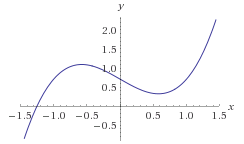
\includegraphics[width=0.48\textwidth]{newtonfail}
  \end{center}
  \caption{$f(x) = x^3 - x + \frac{\sqrt{2}}{2}$}
\end{wrapfigure}

\section{Main Idea of the Proof}
\label{sec:main-idea-proof}

\section{Diophantine Differential Equations}
\label{sec:dioph-diff-equat}

\section{Solving Equations}
\label{sec:solving-equations}

\section{Conclusion}
\label{sec:conclusion}



\end{document}

%%% Local Variables:
%%% mode: latex
%%% TeX-master: t
%%% End:
